\section{\sys Design}\label{sec:design}

%\begin{figure}[t]
    \centering
    %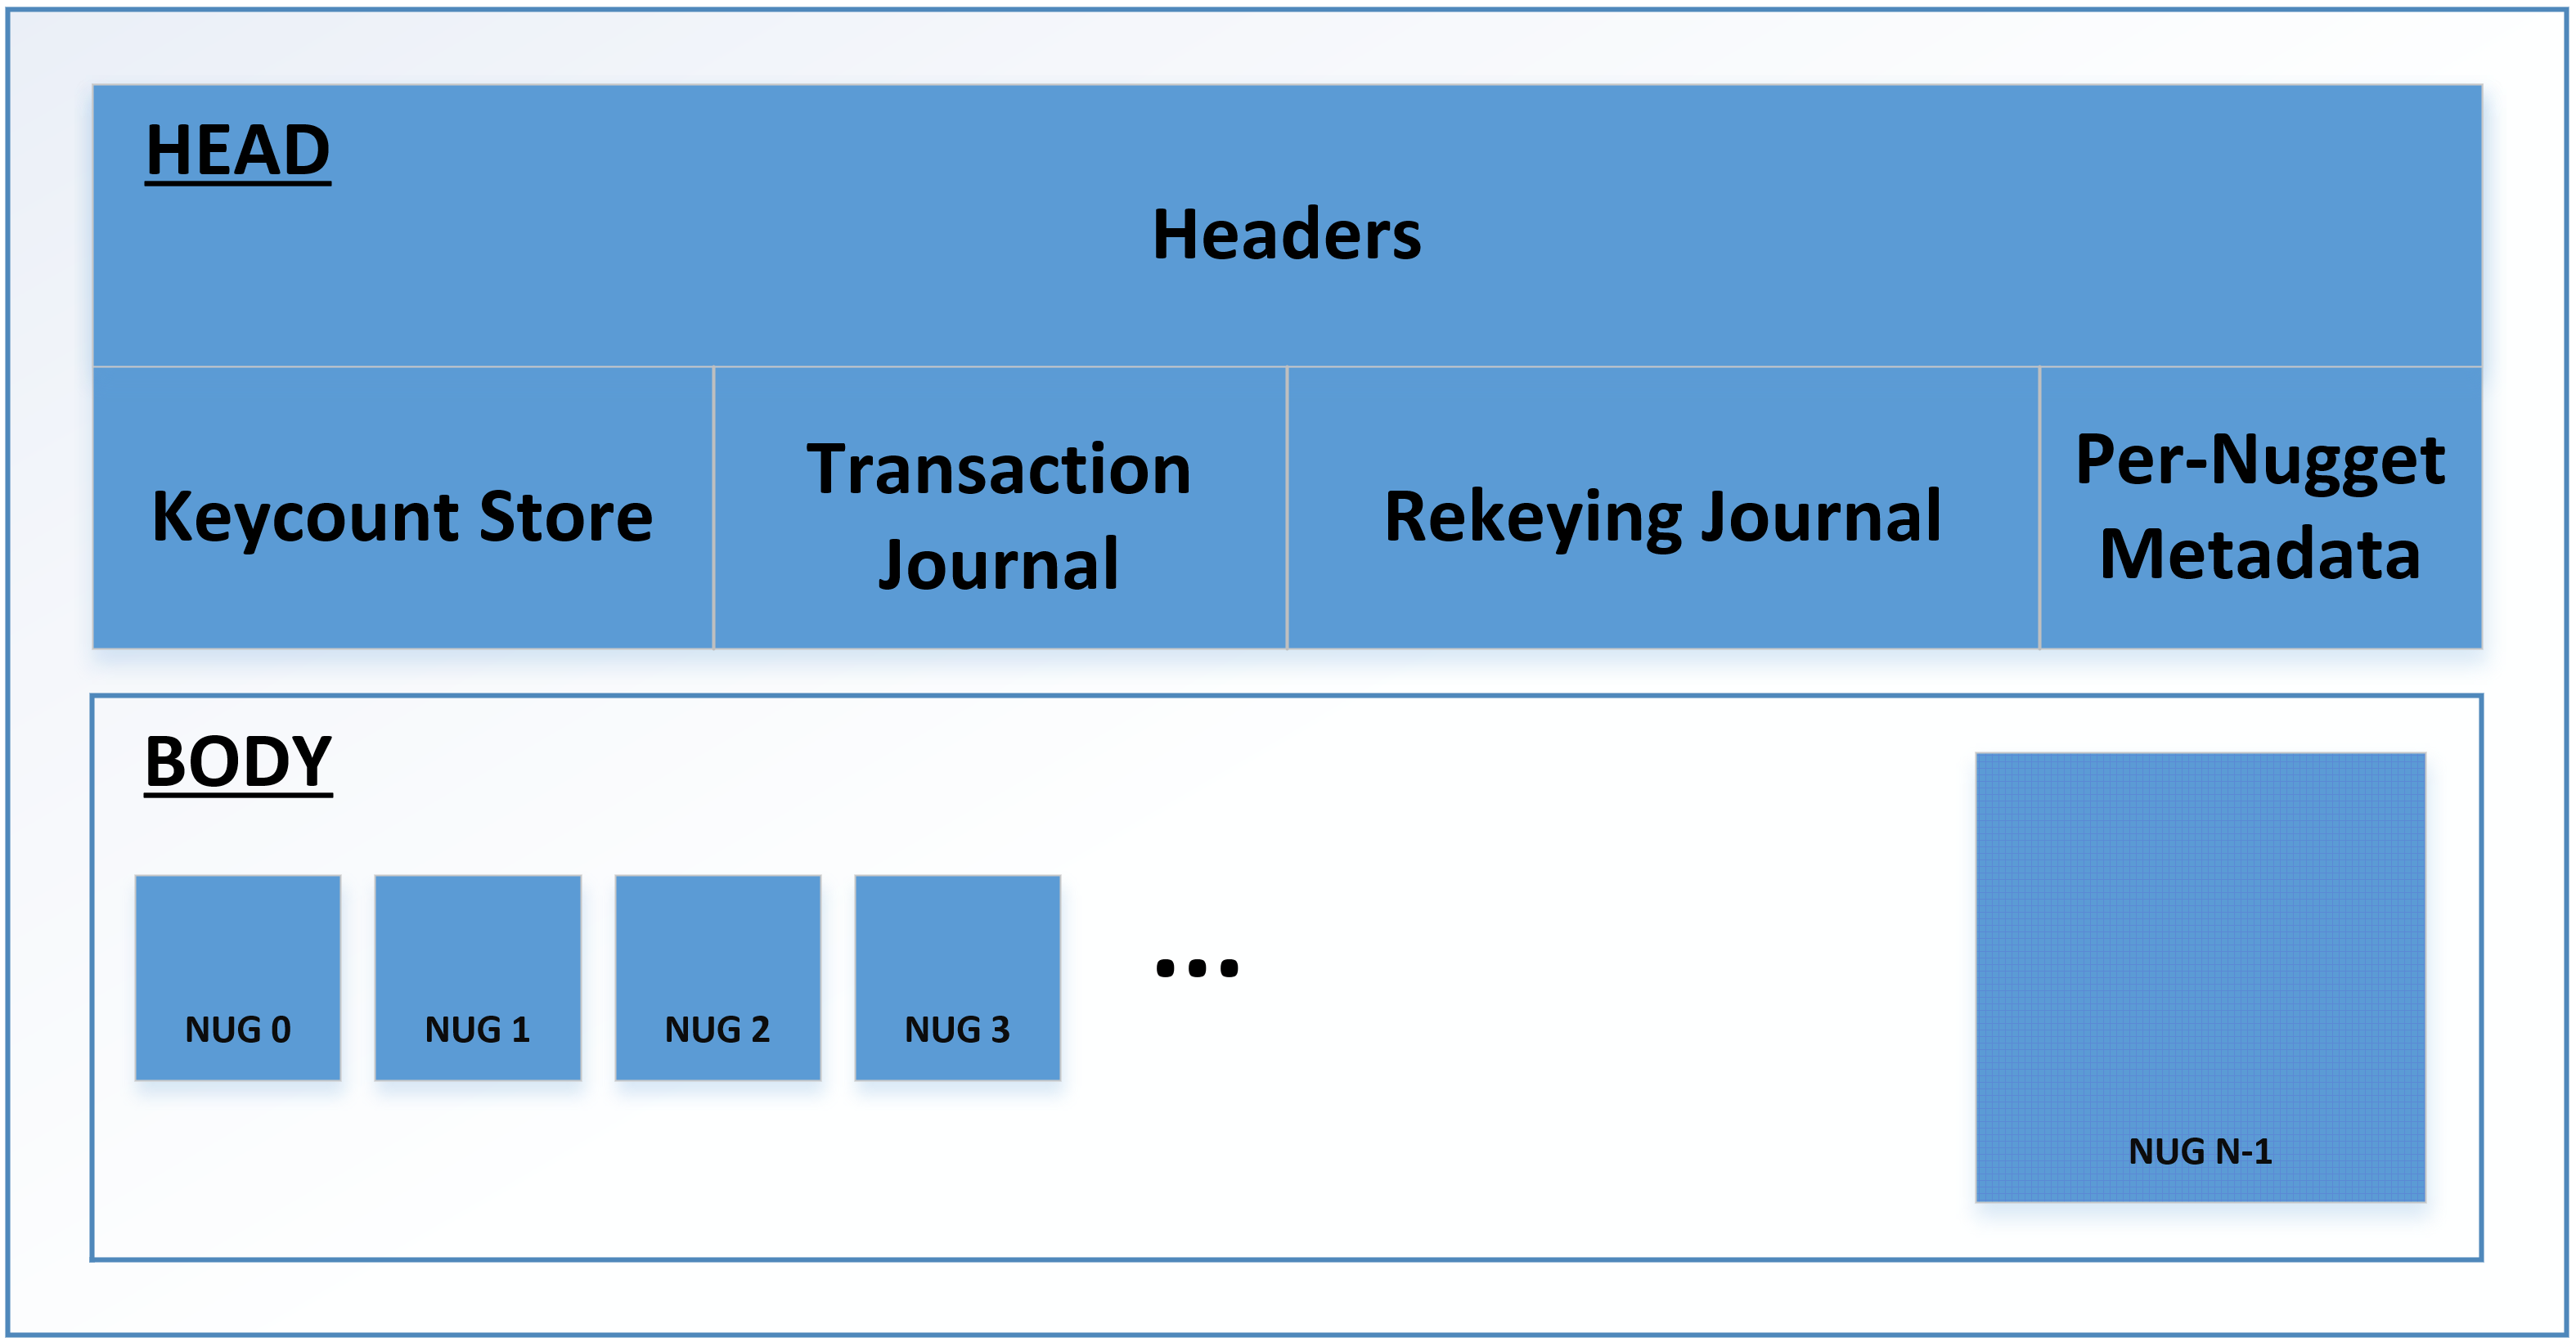
\includegraphics[width=\linewidth]{backstore.png}
    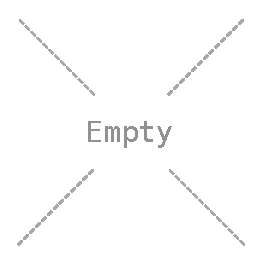
\includegraphics[height=1in]{empty.eps}
    \mycaption{fig:backstore}{Layout of \sys's drive layout.}{The figure is
    explained in Section \ref{..}.}
\end{figure}


% About: basics, dependent
\sys is a block layer kernel module that can replace other state-of-the-art
block-level encryption technologies such as the popular dm-crypt. \sys does not
require any modification in the application and only a small modification in the
file system layer to expose the inode-block mapping. The choice to do this at
the block layer is important to ensure the core logic of file systems does not
have to be modified. Just like any other encryption technologies, \sys must have
a unit of en/decryption. In this paper we call it a ``nugget,'' which can be
configured as one or more sequential blocks.

To provide a kernel support for different cipher configurations and live cipher
switching, we must address three key challenges:

\begin{enumerate}

\item We must provide switching models, both that cover temporal and spatial
  nature of storage data and accesses, to support live switching that users
  demand. For this, we introduce the \sysA (Section \ref{x}) component of \sys
  that exposes three switching models to users: forward, selective and mirrored
  switching.

\item We must allow different cipher implementations to be easily integrated to
  \sys, however different ciphers require different types of inputs and outputs
  and often they are tightly integrated to the encrypted data and the on-disk
  data structures that the encryption layer uses. For this, we introduce the
  \sysB (Section \ref{x}) component where we decouple cipher implementations
  from the core encryption algorithm and provide interfaces that allows many
  different encryption algorithms (``crypts'') to be rewritten easily.

\item We must help users understand the tradeoffs of different cipher
  configurations, hence we introduce \sysC (Section \ref{x}), a method that
  attempts to quantify the desirable properties of different cipher
  configurations in several metrics such as the round-trip, randomization and
  expansion costs.

\end{enumerate}

